% =====================================================================
%  Title page — title, author, hero chart with caption.
% =====================================================================
\begin{titlepage}
\centering
\vspace*{1.0cm}

\slayertitle
  {Slayer 150 1.01:\\ choosing a training recipe with decision rules\\ fixed before each result}%
  {Arkadiusz Słota, Fabryka AI}%
  {Draft, 7 October 2026 --- training in progress}

\vspace{0.8cm}

\begin{figure}[h]
  \centering
  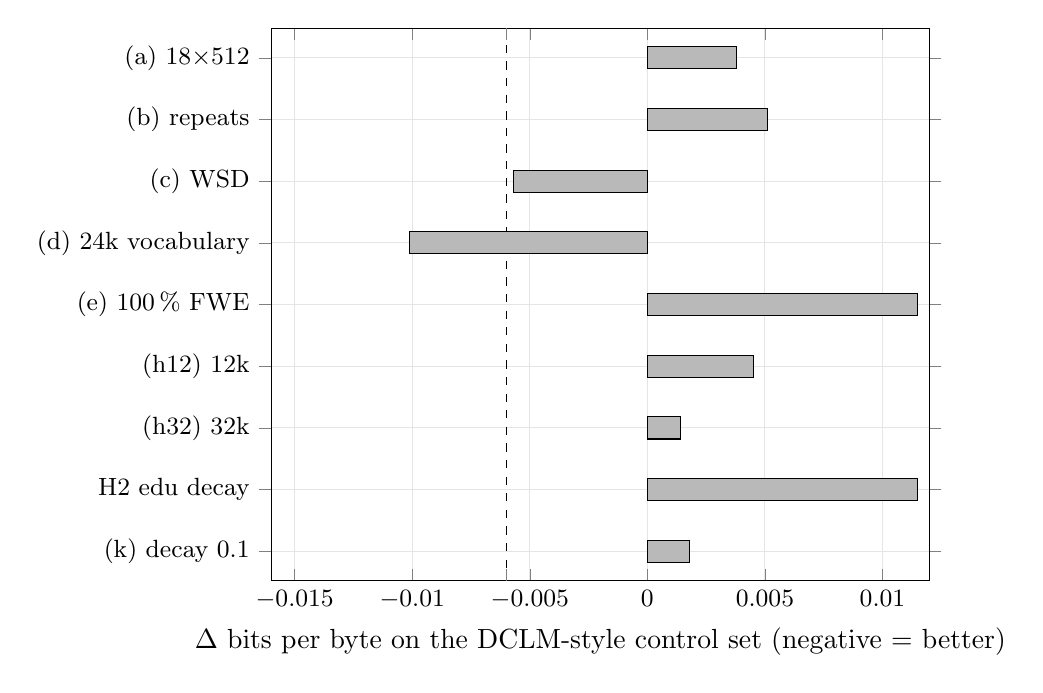
\begin{tikzpicture}
    \begin{axis}[
        xbar, width=0.82\linewidth, height=8.6cm,
        xlabel={$\Delta$ bits per byte on the DCLM-style control set (negative = better)},
        xmin=-0.016, xmax=0.012,
        ytick={1,...,9},
        yticklabels={(a) 18$\times$512, (b) repeats, (c) WSD, (d) 24k vocabulary, (e) 100\,\% FWE, (h12) 12k, (h32) 32k, H2 edu decay, (k) decay 0.1},
        scaled x ticks=false, xtick={-0.015,-0.010,-0.005,0,0.005,0.010},
        x tick label style={/pgf/number format/fixed, /pgf/number format/precision=3, font=\small},
        bar width=8pt, enlarge y limits=0.06,
        grid=major, grid style={gray!20},
        extra x ticks={-0.006}, extra x tick labels={}, extra x tick style={grid=major, grid style={black, dashed}},
        y dir=reverse, y tick label style={font=\small},
    ]
      \addplot[fill=gray!55] coordinates {
        (0.0038,1) (0.0051,2) (-0.0057,3) (-0.0101,4) (0.0115,5) (0.0045,6) (0.0014,7) (0.0115,8) (0.0018,9)};
    \end{axis}
  \end{tikzpicture}
  \caption{\textbf{Nine ablations at 64M parameters and 2B tokens, judged by rules written before each result.}
  Bars show the change in bits per byte on the DCLM-style control set against the arm's control; the dashed line
  is the acceptance threshold $-0.006$. Only the 24k vocabulary (d) crossed it. Bars for (e) and H2 are cut at
  $+0.0115$; their true values are $+0.0888$ and $+0.0505$. Values from the verdict files listed in
  \texttt{recipe/}.}
  \label{fig:hero}
\end{figure}

\vfill
{\small Fabryka AI \textperiodcentered{} SlayerLabs \textperiodcentered{} all numbers pinned by SHA-256 to result files}
\end{titlepage}
